%----------------------------------------------------------------------------------------
%	Debug options
%----------------------------------------------------------------------------------------
% chktex-file 2
% chktex-file 8
% chktex-file 11
% chktex-file 13
% chktex-file 18
% chktex-file 36
% chktex-file 39
% chktex-file 44
%----------------------------------------------------------------------------------------
\chapter{Appendix}
%----------------------------------------------------------------------------------------
%	List of Acronyms
%----------------------------------------------------------------------------------------
\section{Acronyms}\label{sec:acronyms}
% # 
% # Usage:
% # \ac{kürzel} = Erstes Mal Langform mit (Kürzel) dann nur noch Kürzel mit Link zum Acronym
% # \acl{kürzel} = gibt nur die Langform der Abkürzung aus mit Link zum Akronym
% # \acp{kürzel} || \aclp{kürzel} = Selbes wie oben nur mit Plural version
% # 
%----------------------------------------------------------------------------------------
%	Debug options
%----------------------------------------------------------------------------------------
% chktex-file 36
% chktex-file 39
% chktex-file 18
% chktex-file 8
% chktex-file 11
%----------------------------------------------------------------------------------------
%	Usage options
%----------------------------------------------------------------------------------------
% \acf{po} (Product Owner (PO))
% \ac{po} (product owner)(po)
% \Ac{po} (Product Owner)(Po)
% \acp{po} (Product Owners)(POs)

\begin{acronym}[HCD]
    \acro{ux}[UX]{User-Expierience}
    \acro{ui}[UI]{User-Interface}
    \acro{po}[PO]{Product Owner}
    \acroplural{po}[POs]{Product Owners}
    \acro{pm}[PM]{project manager}
    \acroplural{pm}[PMs]{project managers}
    \acro{safe}[SAFe]{Scaled Agile Framework}
    \acro{less}[LeSS]{Large-Scale Scrum}
    \acro{agile-manifesto}[Agile Manifesto]{Manifesto for Agile Software Development}
    \acro{asd}[ASD]{Agile Software Development}
    \acro{dod}[DoD]{Defintion of Done}
\end{acronym}

%----------------------------------------------------------------------------------------
%	List of Glossaries
%----------------------------------------------------------------------------------------
\newpage
\printnoidxglossaries%

%----------------------------------------------------------------------------------------
%	List of Interviewees
%----------------------------------------------------------------------------------------
\newpage
\section{List of Participants}\label{app:ListOfParticipants}

\textbf{Normen Möller}\newline
{Freelancer}\newline
\icontext{Xing}{14}{\href{https://www.xing.com/profile/Normen_Moeller/cv}{Normen$\_$Moeller}}{black}

\textbf{Sonja Zuckerstätter BA MSc}\newline
{Content Managerin}\newline
\textit{content garden technologies GmbH}\newline
\icontext{Linkedin}{14}{\href{https://www.linkedin.com/in/sonja-zuckerstaetter}{sonja-zuckerstaetter}}{black}

\textbf{Norman Günther}\newline
{IT Project Manager | Agile Coach}\newline
\textit{BZ.medien Digital}\newline
\icontext{Xing}{14}{\href{https://www.xing.com/profile/Norman_Guenther4/cv}{Norman$\_$Guenther4}}{black}

\textbf{Michael Spiller}\newline
{Senior Agile Coach}\newline
\textit{metafinanz Informationssysteme GmbH}\newline
\icontext{Linkedin}{14}{\href{https://linkedin.com/in/michaelspiller}{michaelspiller}}{black}

\textbf{Mario Hirschfeld}\newline
{Agile Coach} \newline
\textit{L.N. Schaffrath DigitalMedien GmbH}

\textbf{Jean-Pierre Berchez}\newline
{Gesellschafter} \newline
\textit{HLSC GmbH}\newline
\icontext{Linkedin}{14}{\href{https://www.linkedin.com/in/jpberchez/}{jpberchez}}{black}

\newpage
\section{Link to the spreadsheet used for analysis}\label{app:QRCode}
To download the spreadsheet through your Browser, click this link right \textcolor{Violet}{\href{https://github.com/Inf166/mai-joel_maximilian-bachelor_thesis/raw/main/assets/data/data-formated-for-analysis.xlsx}{here}}.

Alternatively, you can scan this QR Code with your phone camera:
\begin{figure}[!ht]
    \makebox[128pt]{
\includegraphics[width=128pt]{./assets/images/qr-code-to-the-spreadsheet-github.png}}
\end{figure}

\section{How to cite this thesis}
\subsection*{BibTex}
\begin{lstlisting}[label={lst:HowToCite}]
@MastersThesis{MaiGrotenKullack2023IttpoS,
author           = {Mai, Joel Maximilian and Groten, Raphaela and Kullack, Sven},
title            = {{Investigating} the theory-practice gap of {Scrum}},
year             = {2023},
month            = {02},
type             = {Bachelor's Thesis},
journal          = {Technische Hochschule Koeln},
keywords         = {scrum, agile software development, framework, methodology, theory-practice gap}
}
\end{lstlisting}

\begin{description}
    \item[MLA] Mai, Joel Maximilian, et al. Investigating the Theory-Practice Gap of Scrum. 02 2023.
    \item[APA] Mai, J. M., Groten, R., \& Kullack, S. (02 2023). Investigating the theory-practice gap of Scrum.
    \item[AMA] Mai JM, Groten R, Kullack S. Investigating the Theory-Practice Gap of Scrum. 02 2023.
    \item[IEEE] J. M. Mai, R. Groten, and S. Kullack, 'Investigating the theory-practice gap of Scrum', 02 2023.
    \item[Harvard] Mai, J. M., Groten, R. and Kullack, S. (02 2023) Investigating the theory-practice gap of Scrum.
    \item[Chicago] Mai, Joel Maximilian, Raphaela Groten, and Sven Kullack. 'Investigating the Theory-Practice Gap of Scrum', 02 2023.
\end{description}
%----------------------------------------------------------------------------------------
%	List of References
%----------------------------------------------------------------------------------------
\bibliographystyle{apacite}
\renewcommand{\refname}{List of References}
\bibliography{bibliography/biblio.bib}

%----------------------------------------------------------------------------------------
%	List of Figures
%----------------------------------------------------------------------------------------
\newpage
\listoffigures
	
%----------------------------------------------------------------------------------------
%	List of Tables
%----------------------------------------------------------------------------------------
%\newpage
%\addcontentsline{toc}{chapter}{List of Tables}
%\listoftables

%\newpage

%----------------------------------------------------------------------------------------
%	Questionnaire
%----------------------------------------------------------------------------------------
%----------------------------------------------------------------------------------------
%	Debug options
%----------------------------------------------------------------------------------------
% chktex-file 1
% chktex-file 2
% chktex-file 8
% chktex-file 11
% chktex-file 13
% chktex-file 18
% chktex-file 26
% chktex-file 36
% chktex-file 39
% chktex-file 44
%----------------------------------------------------------------------------------------
\newpage
\section{Questionnaire}\label{app:Questionnaire}
\einzelantworticon = Single-choice question; \checkboxantworticon = Multiple-choice question

\section*{Über mich}
Ich heiße Joel Maximilian Mai und bin 24 Jahre alt. Zur Zeit studiere ich Medieninformatik an der Technischen Hochschule Köln. Für meine Bachelorarbeit und aus eigenem Interesse beschäftige ich mich viel mit agilen Frameworks, Methoden und ins besondere Scrum. Da ich selbst Webentwickler bin, interessiere ich mich sehr für den besten Weg Software zu entwickeln. 

\section*{Was ist der Grund für die Umfrage?}
Das Thema meiner Bachelorarbeit ist "Investigating the Theory-Practice Gap of Scrum". In der Theorie klingt Scrum sinnvoll und klar. Jedoch werden Frameworks häufig in der Theorie erweitert und für die Anwendung in der Praxis angepasst. Während meiner Literatur Recherche konnte ich viele Gründe und Lösungsansätze für die Herausforderungen aber auch für den Gap identifizieren. Jedoch, um nicht selbst einen Gap zwischen Literatur und Praxis zu erzeugen, benötige ich die Evaluierung meiner Ergebnisse durch eine Umfrage.

\section*{Welchem Zweck soll die Umfrage dienen?}
Mit Ihrer Unterstützung möchte ich mehr über den Gebrauch des Scrum Frameworks in der Praxis erfahren. Ich möchte erfahren, was gut läuft und die von mir in der Literatur identifizierten Probleme hinterfragen und ergänzen. Ich bin interessiert an den Gründen, warum Sie Scrum anwenden und an den Ursachen möglicher Herausforderungen. 

\section*{Danke für Ihre Teilnahme}
Ich danke Ihnen herzlich für die Teilnahme. Dieses Thema interessiert mich ganz besonders. Die Ergebnisse dieser Studie und der Arbeit werden hoffentlich anderen begeisterten Menschen bei ihrem Weg helfen.

\textit{Diese Umfrage dauert etwa 15 Minuten.}

\section*{Über Sie}
In diesem Abschnitt erfasse ich die zuvor genannten Rahmendaten um später in der Analyse Zusammenhänge zwischen der Position und Erfahrung und den beschriebenen Herausforderungen herzustellen.

\section*{Wie lautet ihre aktuelle Berufsbezeichnung?}
\kurzantwort

\section*{Wie lange arbeiten Sie schon in dem Bereich? (in Jahren)}
\kurzantwort

\section*{Hatten Sie bereits Erfahrung in einer anderen Rolle/Position, wenn ja, in welchen?}
\kurzantwort

\section*{Unternehmen und Team}
In diesem Abschnitt erfasse ich Rahmendaten über die Unternehmen um später Zusammenhänge zwischen der Größe, der Anzahl der Herausforderungen aber auch welche Herausforderungen besonders häufig auftreten herzustellen.

\section*{Wie groß ist das Unternehmen in dem Sie eingestellt sind aktuell?}
\einzelantwort{Kleinstunternehmen (weniger als 10 Personen)}
\einzelantwort{Kleinunternehmen (10-49 Personen)}
\einzelantwort{mittleres Unternehmen (50-249 Personen)}
\einzelantwort{Großunternehmen (mehr als 250 Personen)}

\section*{Welches Produkt bietet ihr Unternehmen an? (eigene Software, Webseiten für Kunden, ...)}
\kurzantwort

\section*{Wie groß ist Ihr aktuelles Team?}
\kurzantwort

\section*{An wie vielen Projekten arbeitet Ihr Team durchschnittlich gleichzeitig?}
\kurzantwort

\section*{Agile Frameworks, Agile Methoden}
Mir ist bewusst, dass viele Unternehmen nicht ausschließlich Scrum verwenden, daher erfasse ich in diesem Abschnitt die Abweichung von dem eigentlichen Scrum Guide.

\section*{Welche der folgenden agilen Methoden nutzen Sie?}
\einzelantwort{Scrum}
\einzelantwort{Scrumban}
\einzelantwort{Scrum-eXtreme Programming Hybrid}
\einzelantwort{Kanban}
\einzelantwort{Iterative}
\einzelantwort{Lean Thingking}
\einzelantwort{Weitere ...}

\section*{Für welches der folgenden Frameworks hat sich Ihr Unternehmen entschieden?}
\einzelantwort{Scrum (Nach Jeff Sutherland und Ken Schwaber)}
\einzelantwort{Disciplined Agile}
\einzelantwort{Scrums of Scrums (Jeff Sutherland)}
\einzelantwort{Nexus}
\einzelantwort{Scrum@Scale}
\einzelantwort{Enterprise Scrum}
\einzelantwort{Scaled Agile Framework (SAFe)}
\einzelantwort{Large Scale Scrum (LeSS)}
\einzelantwort{Agile Portfolio Management}
\einzelantwort{Weitere ...}

\section*{Wie sehr hält sich Ihr Unternehmen dabei an das Framework?}
\skalarvonbis{1}{10}{gar nicht}{strikt nach Lehrbuch}

\section*{An welchen Stellen weicht Ihr Unternehmen von der Theorie ab?}
\langantwort

\section*{Für wie gravierend halten Sie den Einfluss dieser Abweichung auf den Erfolg der Scrum Integration?}
\skalarvonbis{1}{5}{unbedeutend}{gravierend}

\section*{Hatten Sie bereits Erfahrung mit einem der anderen genannten Frameworks?}
\checkboxantwort{Scrum (Nach Jeff Sutherland und Ken Schwaber)}
\checkboxantwort{Disciplined Agile}
\checkboxantwort{Scrums of Scrums (Jeff Sutherland)}
\checkboxantwort{Nexus}
\checkboxantwort{Scrum@Scale}
\checkboxantwort{Enterprise Scrum}
\checkboxantwort{Scaled Agile Framework (SAFe)}
\checkboxantwort{Large Scale Scrum (LeSS)}
\checkboxantwort{Agile Portfolio Management}
\checkboxantwort{Weitere ...}

\section*{Welche der folgenden Methoden nutzt Ihr Unternehmen aktiv?}
\checkboxantwort{Daily Stand-Up}
\checkboxantwort{Retrospektiven}
\checkboxantwort{Sprint/Iterations Review}
\checkboxantwort{Sprint/Iterations Planning}
\checkboxantwort{Backlog Refinement}
\checkboxantwort{Digital Kanban Board}
\checkboxantwort{User Stories und oder Epics}
\checkboxantwort{Story Points}
\checkboxantwort{Planning Poker / Schätzungen}
\checkboxantwort{Häufige Releases}
\checkboxantwort{Work in Progress Limits}
\checkboxantwort{Physikalisches Kanbanboard}
\checkboxantwort{Weitere ...}

\section*{Wie lange dauert ein Sprint bei Ihnen in Wochen? (0 für keine Sprints)}
\einzelantwort{0}
\einzelantwort{1}
\einzelantwort{2}
\einzelantwort{3}
\einzelantwort{4}
\einzelantwort{Weitere ...}

\section*{Bestandsaufnahme: Scrum}
Um jetzt aber doch bessere Schlüsse ziehen zu können um den Gap von Scrum zu definieren, erfasse ich im folgenden Abschnitt explizite Daten zu der Erfahrung mit Scrum und das Erlernen des Frameworks.

\section*{Wie lange arbeitet Ihr Team bereits mit Scrum?}
\einzelantwort{Aktuell noch in der Testphase}
\einzelantwort{Kürzer als ein Jahr}
\einzelantwort{1-2 Jahre}
\einzelantwort{3-5 Jahre}
\einzelantwort{5 Jahre und mehr}

\section*{Wie lange arbeiten Sie schon mit Scrum? (in Jahren)}
\kurzantwort

\section*{Haben Sie schon einmal den Scrum Guide gelesen?}
\einzelantwort{Ja}
\einzelantwort{Teilweise}
\einzelantwort{Nein}

\section*{Wenn Sie sich bereits mit einer Veröffentlichung des Scrum Guides beschäftigt haben, mit welcher? (Jahr genügt)}
\kurzantwort

\section*{Welche Abteilungen nutzen Scrum in Ihrem Unternehmen? (Projektmanagement, HR, UX, UI, Konzeption, Entwicklung...)}
\langantwort

\section*{Wie viele Teammitglieder haben eine aktive Auseinandersetzung mit der Theorie von Scrum abgeschlossen und somit ein ausgeprägtes Verständnis?}
\kurzantwort

\section*{Welche Quelle halten Sie für Wertvoll um sich das Scrum Framework anzueignen?}
\langantwort

\section*{Wenn Sie ein Zertifakt für Scrum oder eine der Rollen besitzen, von welcher Quelle?}
\kurzantwort

\section*{Wie würden Sie die Expertise bewerten, die ein solches Zertifikat vermittelt?}
\skalarvonbis{1}{5}{Basiswissen}{Experte in dem Framework/Rolle}

\section*{Was waren Gründe oder Ursachen für ihr Unternehmen, das Framework Scrum zu wählen?}
\langantwort

\section*{Zu dem Gap in der Praxis}
Dieser Abschnitt ist wahrscheinlich der wichtigste von allen. Er bietet Ihnen die Möglichkeit den Erfolg der Integration von Scrum einzuschätzen und die wichtigsten Herausforderungen als auch Lösungsansätze sowie Tipps zu äußern. 

\section*{Wie würden Sie den Erfolg der Integration von Scrum in Ihrem Unternehmen bewerten?}
\skalarvonbis{1}{8}{Gescheitert}{Voller Erfolg}

\section*{Was sind die Herausforderungen der Integration von Scrum gewesen?}
\langantwort

\section*{Was waren Lösungsansätze mit denen Ihr Unternehmen versucht hat die Herausforderungen zu lösen?}
\langantwort

\section*{Welche Herausforderungen blieben bis heute bestehen?}
\langantwort

\section*{Welche Ratschläge würden Sie anderen Unternehmen, Teams oder Kollegen mitgeben um die Integration und Adaption von Scrum zu erleichtern?}
\langantwort

\section*{Halten Sie Scrum für ungeeignet für Ihren Anwendungszweck?}
\einzelantwort{ungeeignet}
\einzelantwort{projektabhängig}
\einzelantwort{geeignet}

\section*{Welche Rollen oder Methoden wurden von dem Alten mit in den neuen Prozess übernommen und warum? (z.B. bei Wasserfall -> Scrum, könnte das Projektmanager sein oder Anforderungsmanagement)}
\langantwort

\section*{Wer leitete Ihre Transformation/den Übergang zu Scrums Methoden? (Rolle/Position)}
\langantwort

\section*{Wie schätzen Sie die Selbstorganisation und das Selbstmanagement Ihres Teams ein?}
\skalarvonbis{1}{5}{von außen kontrolliert}{selbst organisiert}

\section*{Wie hoch ist Ihre Motivation Scrum durch ein anderes Framework zu ersetzen?}
\skalarvonbis{1}{5}{niedrig}{hoch}

\section*{Welches Framework empfehlen Sie alternativ?}
\kurzantwort

\section*{Was wären die Gründe für die Anwendung eines anderen Frameworks?}
\checkboxantwort{Jobwechsel (Neues Team arbeitet nicht agil)}
\checkboxantwort{Jobwechsel (Kein Programmierer mehr)}
\checkboxantwort{Management war im Weg}
\checkboxantwort{Aktueller Prozess ist ähnlich aber nicht agil}
\checkboxantwort{Der Versuch Agilität zu praktizieren schlug fehl}
\checkboxantwort{Die Koordination mit nicht agilen Teams war schwierig}
\checkboxantwort{Die Projekte litten unter schlechtem Design}
\checkboxantwort{Weitere ...}

\section*{Bekannte Herausforderungen und deren Lösungsansätze}
Dieser Teil ist fast so bedeutsam wie der vorherige. Hier möchte ich Ihnen zeigen welche Erkenntnisse ich durch die Literatur erlangen konnte. Ich brauch jedoch Ihre Hilfe dabei mir zu bestätigen welche der Gründe, Herausforderungen und Lösungsansätze tatsächlich in Ihrer Praxis stattfanden. Gerne dürfen Sie mir im Anschluss an die Umfrage Fragen zu den einzelnen Punkten stellen.

\section*{Welche der folgenden Gründe waren es, die zur Integration von Scrum in Ihrem Unternehmen gesorgt haben?}
\checkboxantwort{Vorhersehbarkeit, Transparenz und Sichtbarkeit}
\checkboxantwort{Frühe Risiko-Reduktion}
\checkboxantwort{Schnelleres Deployment an den Kunden oder Testumgebung}
\checkboxantwort{Schnelleres Return on Investment}
\checkboxantwort{Schnelleres Feedback von echten Nutzern}
\checkboxantwort{Kundenzufriedenheit ist verbessert}
\checkboxantwort{Reibungslosere Teamarbeit}
\checkboxantwort{Software Qualitätsverbesserung}
\checkboxantwort{Effektivitätsverbesserung}
\checkboxantwort{Mehr automatisiertes Testing}
\checkboxantwort{Produktivitätsverbesserung}
\checkboxantwort{Bessere Produkte für Kunden und Nutzer entwickeln}
\checkboxantwort{Verbessern von Reaktion auf sich verändernde Anforderungen und Prioritäten}
\checkboxantwort{Verbesserung von Einigkeit von Unternehmen und Entwicklern}
\checkboxantwort{Verbesserte Moral im Team}
\checkboxantwort{Anforderungsänderungen fallen leichter}
\checkboxantwort{Management entschied sich dafür}

\section*{Welche der folgenden Herausforderungen hatte Ihr Unternehmen bei der Integration von Scrum?}
\checkboxantwort{Es wurde nicht geprüft ob agile Software Entwicklung sinnvoll für das Unternehmen ist}
\checkboxantwort{Langsame Entscheidungsfindung. Zunächst ist nicht nur unklar wer die Entscheidungen zu treffen hat, aber auch die Informationsweitergabe erfolgt träge oder passiv.}
\checkboxantwort{Fehlendes Commitment sich ganz und gar der agilen Software Entwicklung zu verschreiben.}
\checkboxantwort{Es gibt keinen gemeinsamen Willen mehr über Scrum und agiler Software Entwicklung zu lernen}
\checkboxantwort{Die Integration von der agilen Kultur endete mit der Bekanntmachung von Scrum im Unternehmen}
\checkboxantwort{Fehlendes agiles Mindset und Kultur. Die Meinungen über die Sinnhaftigkeit eines agilen Mindsets wird nicht von allen geteilt}
\checkboxantwort{Zu viele Personen involviert. Viele verschiedene Meinungen über was Scrum ist und wie es integriert werden sollte}
\checkboxantwort{Scrum wurde von einen auf den anderen Tag etabliert und hat viel Schaden angerichtet}
\checkboxantwort{Es fehlenen erfahrene Mitarbeiter}
\checkboxantwort{Das Unternehmen legt keinen Wert darauf zu messen, Herausforderungen zu identifizieren und Lösungen für diese zu finden}
\checkboxantwort{Scrum wurde nur in der Entwicklung Integriert und der Rest des Unternehmens folgt dem Wasserfall Modell}
\checkboxantwort{Der Geschäftsführung ist es gleichgültig was das agile Mindset ist und sieht keinen Grund selbst Veränderungen im Unternehmen anzuordnen}
\checkboxantwort{Das Management will keine Kontrolle über die Teams abgeben und greift in die Arbeit ein}
\checkboxantwort{Das Management limitiert den Einfluss des Scrum Masters oder eines Agile Coaches}
\checkboxantwort{Das Management entschied agil zu werden ohne Abstimmung im Team}
\checkboxantwort{Das Management mikro-managet das Entwickler-Team}
\checkboxantwort{Der Scrum Master hat nicht die Qualifikation um bei der Integration von Scrum im Unternehmen zu helfen}
\checkboxantwort{Kollaboration und Koordination. Das Team ist verteilt (remote) und Austausch findet zu selten statt.}
\checkboxantwort{Das Entwickler Team greift nicht auf die Expertise ihrer Kollegen zurück}
\checkboxantwort{Das Team teilt nicht die für Scrum notwendige intrinsische Motivation}
\checkboxantwort{Das Team hat nicht die Erlaubnis entscheidungen selbst zu treffen}
\checkboxantwort{Das Team hat nicht das selbe Ziel wie das Unternehmen}
\checkboxantwort{Das Team kennt sich nicht gut genug}
\checkboxantwort{Das Team arbeitet nicht häufig zusammen sondern mehr parallel zueinander}
\checkboxantwort{Es wird nicht regelmäßig für die Inkremente des Produkts Kunden-/Nutzerfeedback gesammelt}
\checkboxantwort{Es wird kein Budget freigegeben für Fortbildungen zur Integration von agiler Software Entwicklung}
\checkboxantwort{Die Räumlichkeiten und Zusammenarbeit hat sich nicht verändert um Scrum-basiertes Arbeiten zu ermöglichen}
\checkboxantwort{Informationen über den Projektstatus werden nicht regelmäßig kommuniziert}
\checkboxantwort{Die Backlogs wird nicht konsequent und effektiv priorisiert}
\checkboxantwort{Schlüsselpositionen im Unternehmen sind nicht von Personen besetzt die die notwendige Qualifikation besitzen}
\checkboxantwort{Alte Positionen wurden nicht durch die neuen Rollen und Weiterbildungen ersetzt}
\checkboxantwort{Die Anzahl der Meetings reduzierte die Produktivität}
\checkboxantwort{Es gab kein Upfront-Design / Konzeption und oder blieb bei einem niederen Design}
\checkboxantwort{Entwickler die später am Projekt arbeiten, sind nicht Teil des Teams welches die Planung und Konzeption vollzieht}
\checkboxantwort{Erfolg des Projekts wird nicht angemessen für ein agiles Projekt gemessen und fehlinterpretiert}
\checkboxantwort{Kunden und Nutzer werden nicht die Entwicklung mit einbezogen}
\checkboxantwort{Kunden verstehen den Sinn von Konzeption und Anforderungsermittlung}
\checkboxantwort{Der Kunde hält agile Software Entwicklung für riskanter und versteht nicht die Vorteile}

\section*{Welche der folgenden Lösungsansätze hatte auch Ihr Unternehmen versucht?}
\checkboxantwort{Scrum nach Lehrbuch für bestimmte Zeit durchführen}
\checkboxantwort{Geschäftsführung um Rückendeckung für die Integration und Durchführung bitten und schriftlich festhalten}
\checkboxantwort{Training in agile und Scrum für alle Beteiligten}
\checkboxantwort{Training in Feedback- und Kommunikations-Kulur für alle Beteiligten}
\checkboxantwort{Enhancement-Sprints für Low-Prio Backlog Items}
\checkboxantwort{Concept Sprint(s) mit Kunden vor den eigentlichen Development-Sprints}
\checkboxantwort{Team entscheidet welches Framework/Methodologie geeignet ist}
\checkboxantwort{Kunde / Produkt Owener + Business Value (Estimation) entscheiden prio}
\checkboxantwort{Inspect-Adapt Zyklus(Retrospektiven) für die Scrum Integration wird kontinuierlich fortgeführt}
\checkboxantwort{Es wird nicht länger in Abteilungen gedacht sondern in Projektteams und Rollen}
\checkboxantwort{Keine Demos, Kunden nutzen/testen das aktuelle Produkt/Release}
\checkboxantwort{Mittleres Management lernt neue Aufgaben kennen und gibt Kontrolle ab}
\checkboxantwort{Jemand mit Erfahrung und umfassendem Wissen leitet die Transformation und begleitet diese}
\checkboxantwort{Daily Stand-Ups dienen zur Koordination für den kommenden Tag und es werden Probleme beseitigt die dem bestmöglichstem Tag im Weg stehen}
\checkboxantwort{Teams werden nach dem Dreyfus-Squared Model gepaart um bestmöglichste Ergebnisse zu erzielen}
\checkboxantwort{Der aktuelle Projekt Status wird vom Teamleiter im Daily-Standup kurz am Anfang präsentiert}
\checkboxantwort{Die Geschäftsführung kommuniziert strategische und operative Ziele transparent}
\checkboxantwort{Teammitglieder die an zusammenhängenden Teilen eines Produkts arbeiten, arbeiten im engen Austausch zusammen}
\checkboxantwort{Jeder Sprint sollte ein MVP als Ergebnis haben, welches von Kunden und Nutzern getestet werden kann}
\checkboxantwort{Nicht Abteilungen sitzen beisammen, sondern Projektteams}
\checkboxantwort{Nach einem Konzept-Workshop wird ein Design-Konzept Sprint durchgeführt welcher das Konzept in erste Prototypen überführt und zur Weiterentwicklung des Produkts beiträgt}
\checkboxantwort{Im besten Fall ist ein Kunde anwesend um das Produkt unter Beobachtung zu testen, um schnell Anpassungen an den Anforderungen vornehmen zu könnnen, substitutiv kann auch Remote getestet werden}
\checkboxantwort{Die Kunden wurden über die Vorteile von Scrum und agiler Software Entwicklung zu Beginn der Vertragsverhandlungen in Kenntnis gesetzt und eventuell Beispiele genannt bekommen}

\section*{Welche Folgen von agiler Transformation treffen auf Ihr Unternehmen zu?}
\checkboxantwort{Verbesserte Vorhersehbarkeit, Transparenz und Sichtbarkeit}
\checkboxantwort{Frühe Risiko-Reduktion}
\checkboxantwort{Schnelleres Deployment an den Kunden oder Testumgebung}
\checkboxantwort{Schnelleres Return on Investment}
\checkboxantwort{Schnelleres Feedback von echten Nutzern}
\checkboxantwort{Kundenzufriedenheit ist verbessert}
\checkboxantwort{Reibungslosere Teamarbeit}
\checkboxantwort{Software Qualitätsverbesserung}
\checkboxantwort{Effektivitätsverbesserung}
\checkboxantwort{Mehr automatisiertes Testing}
\checkboxantwort{Produktivitätsverbesserung}
\checkboxantwort{Bessere Produkte für Kunden und Nutzer entwickeln}
\checkboxantwort{Verbessern von Reaktion auf sich verändernde Anforderungen und Prioritäten}
\checkboxantwort{Verbesserung von Einigkeit von Unternehmen und Entwicklern}
\checkboxantwort{Verbesserte Moral im Team}
\checkboxantwort{Anforderungsänderungen fallen leichter}

\section*{Ihre Anmerkungen}
Wenn Sie das Gefühl haben, dass Sie gerne noch mehr zu dem Thema sagen möchten haben Sie hier die 
Gelegenheit dazu...

\section*{Haben Sie noch andere Gründe für den Theorie-Praxis Gap von Scrum?}
\langantwort

\section*{Wollen Sie die Quellen für diese Umfrage sehen?}
\einzelantwort{Ja}
\einzelantwort{Nein}

\section*{Möchten Sie für Rückfragen zu Ihren Antworten Ihre Email-Adresse angeben?}
\kurzantwort

\section*{Möchten Sie in meiner Abschlussarbeit als Interviewpartner genannt werden? (Andernfalls bleiben Sie anonym)}
\einzelantwort{Ja}
\einzelantwort{Nein}

\section*{Für die Nennung geben Sie bitte folgende Daten an:}
Titel Vorname Nachname\newline
Aktuelle Position in den Unternehmen\newline
Aktuelles Unternehmen für das Sie arbeiten\newline
(optional) Einen Link zu Ihrem LinkedIn/Xing/... Profil\newline
\langantwort

\section*{Möchten Sie nach Veröffentlichung der Abschlussarbeit benachrichtigt werden um sich die Ergebnisse durchzulesen?}
\einzelantwort{Ja}
\einzelantwort{Nein}


%----------------------------------------------------------------------------------------
%	Questionnaire Results
%----------------------------------------------------------------------------------------
%----------------------------------------------------------------------------------------
%	Debug options
%----------------------------------------------------------------------------------------
% chktex-file 1
% chktex-file 2
% chktex-file 8
% chktex-file 11
% chktex-file 13
% chktex-file 18
% chktex-file 26
% chktex-file 36
% chktex-file 39
% chktex-file 44
%----------------------------------------------------------------------------------------
\newpage
\section{Questionnaire results}\label{app:QuestionnaireResults}
\responsecount = Response count; \openresponse = Open answer of an Interviewee

Some of the results were not easily printable, therefore they are appended as graphs after the questions that were able to print. For the raw data please download the spreadsheet linked in section~\fancyref{app:QRCode}.

\section*{Wie lautet ihre aktuelle Berufsbezeichnung?}
\begin{description}
    \item[2 \responsecount] Agile Coach
    \item[1 \responsecount] Scrum Trainer / Agile Coach / Geschäftsführer
    \item[1 \responsecount] QA Consultant
    \item[1 \responsecount] Projektmanager/PO und Programmierer (selbstständig)
    \item[1 \responsecount] Consultant (Projektmanagement)
    \item[1 \responsecount] IT Project Manager
    \item[1 \responsecount] Softwareentwickler
    \item[1 \responsecount] Berater
    \item[1 \responsecount] Projektmanagement
    \item[1 \responsecount] Content Manager
    \item[1 \responsecount] Referent Entgelt
\end{description}

\section*{Wie lange arbeiten Sie schon in dem Bereich? (in Jahren)}
\begin{description}
    \item[2 \responsecount] 1 Jahr
    \item[2 \responsecount] 10 Jahre
    \item[1 \responsecount] 2 Jahre
    \item[1 \responsecount] 5 Jahre
    \item[1 \responsecount] 6 Jahre
    \item[1 \responsecount] 12 Jahre
    \item[1 \responsecount] 13 Jahre
    \item[1 \responsecount] 15 Jahre
    \item[1 \responsecount] 22 Jahre
    \item[1 \responsecount] 25 Jahre
\end{description}

\section*{Hatten Sie bereits Erfahrung in einer anderen Rolle/Position, wenn ja, in welchen?}
\begin{description}
    \item[3 \responsecount] Ja
    \item[1 \responsecount] Softwareentwicklung
    \item[1 \responsecount] (Senior) Business Consultant, IT Projekt Manager, Engagement Manager, IT Transformation Manager, Versicherungskauffrau
    \item[1 \responsecount] Teamleitung, Abteilungsleitung, Anforderungs-/Qualitätsmanagement
    \item[1 \responsecount] Administration / Entwicklung
    \item[1 \responsecount] Verwicherubngskauffrau
    \item[1 \responsecount] Berater, Enterprise Architekt, Trainer
    \item[1 \responsecount] Geschäftsführer, Country Manager Germany, Vertriebsmitarbeiter, Technischer Sales Support
    \item[1 \responsecount] Scrum Master, Agile Coach
    \item[1 \responsecount] Nein
\end{description}

\section*{Wie groß ist das Unternehmen in dem Sie eingestellt sind aktuell?}
\begin{description}
    \item[5 \responsecount] Großunternehmen (mehr als 250 Personen)
    \item[3 \responsecount] Kleinstunternehmen (weniger als 10 Personen)
    \item[3 \responsecount] Kleinunternehmen (10-49 Personen)
    \item[1 \responsecount] Mittleres Unternehmen (50-249 Personen)
\end{description}

\section*{Welches Produkt bietet ihr Unternehmen an? (eigene Software, Webseiten für Kunden, ...)}
\begin{description}
    \item[1 \responsecount] ein Produkt für die Industrie
    \item[1 \responsecount] Dienstleistung
    \item[1 \responsecount] Dienstleistung zu agilen Themen
    \item[1 \responsecount] Versicherungen
    \item[1 \responsecount] Service dienstleistungen für Entwicklung bis hin zu Marketing
    \item[1 \responsecount] Training, Workshop und 1:1 für Führungskräfte
    \item[1 \responsecount] Webseiten, Apps, Intranet, individual Entwicklung
    \item[1 \responsecount] Webbasierte Lösungen für Kunden
    \item[1 \responsecount] Webseite, Digitale Produkte
    \item[1 \responsecount] Websites und maßgeschneiderte Softwatelösungen
    \item[1 \responsecount] Content Marketing, eigene Software zur Distribution
    \item[1 \responsecount] Software
\end{description}

\section*{Wie groß ist Ihr aktuelles Team?}
\begin{description}
    \item[2 \responsecount] 5
    \item[1 \responsecount] 0
    \item[1 \responsecount] 1
    \item[1 \responsecount] 2
    \item[1 \responsecount] 6
    \item[1 \responsecount] 7
    \item[1 \responsecount] 8
    \item[1 \responsecount] 13
    \item[1 \responsecount] 20
    \item[1 \responsecount] Programm größe / Aktuelles Projekt 200+. Anzahl der Leute in den Teams mit denen ich Arbeite 20 insgesamt
    \item[1 \responsecount] 32
\end{description}

\section*{An wie vielen Projekten arbeitet Ihr Team durchschnittlich gleichzeitig?}
\begin{description}
    \item[2 \responsecount] 4
    \item[2 \responsecount] 2-3
    \item[2 \responsecount] 1
    \item[1 \responsecount] Jedes Team an je einem Projekt zur gleichen Zeit
    \item[1 \responsecount] 0
    \item[1 \responsecount] 5
    \item[1 \responsecount] 6-8
    \item[1 \responsecount] 7
    \item[1 \responsecount] 12
\end{description}

\section*{Welche der folgenden agilen Methoden nutzen Sie?}
\begin{description}
    \item[2 \responsecount] Scrum
    \item[2 \responsecount] Kanban
    \item[1 \responsecount] Scrumban
    \item[1 \responsecount] SAFe
    \item[1 \responsecount] Das Beste aus allen Welten: klassisch trifft agil und Methoden, die bisher keiner kennt
    \item[1 \responsecount] Eine Mischung aus Wasserfall und Scrum.
    \item[1 \responsecount] Agiles Projetkmanagement
\end{description}

\section*{Für welches der folgenden Frameworks hat sich Ihr Unternehmen entschieden?}
\begin{description}
    \item[7 \responsecount] Scrum (Nach Jeff Sutherland und Ken Schwaber)
    \item[2 \responsecount] Scaled Agile Framework (SAFe)
    \item[1 \responsecount] Das Beste aus allen Welten: klassisch trifft agil und Methoden, die bisher keiner kennt
    \item[1 \responsecount] Angepasstes Less
    \item[1 \responsecount] Eher eine agile Herangehensweise um für den Kunden und dem Projekt die richtige Arbeitsweise zu finden.
\end{description}

\section*{An welchen Stellen weicht Ihr Unternehmen von der Theorie ab?}
\begin{itemize}
    \item[\openresponse] An denen, wo es nicht mit der Unternehmenskultur und Unternehmenswerten übereinstimmt. An denen, wo das Framework zu starre Grenzen setzt und damit eher Mehraufwand produziert als die Zusammenarbeit fördert. Ich habe über 20 Jahre Berufserfahrung, davon 10 Jahre in der IT Beratung, daher kenne ich die guten und schlechten Seiten von allen gängigen Methoden und Frameworks
    \item[\openresponse] Rollenverteilung (PO häufig nicht verfügbar oder muss anderweitig, zB durch internen Projektmanager, vertreten werden.) - Ereignisse / Meetings (Häufig nicht in Gänze durchführbar, da Kunden nicht immer bereit sind diese vollumfänglich zu bezahlen und an diesen Stellen sparen möchte) - Daily Scrum wird häufig nur wöchentlich durchgeführt
    \item[\openresponse] Wenn Kunde und/oder Projekt es nicht hergeben, wird komplett klassisch gearbeitet. Dies betrifft kleine überschaubare Projekte, wo agil eher mit Kanonen auf Spatzen schießen wäre. Vor allem wenn der Kunde keinen Mehrwert sieht, sind jegliche Diskussionen überflüssig und kosten nur unnötig Zeit.
    \item[\openresponse] Nach der Lehrbuch SCRUM Phase (3-6 Sprints pro Team) darf das Team selbstständig per Retro Anpassungen vornehmen, die auch SCRUM nach Lehrbuch verändern können. Das sind in der Regel kleine Stellschrauben.
    \item[\openresponse] Kein Business Value an Objectives, Keine Lean Business Cases, Ungenügende Einbindung der Business Owner, Kein Continuous Deployment, Keine Einbeziehung Feedback da verzögerte System Demo
    \item[\openresponse] Hauptächlich Rollenverteilung (es gibt Überschneidungen) den Rest versuchen wir nach Lehrbuch, haben aber keinen ausgebildeten Scrum Master
    \item[\openresponse] Planung und ausführung der arbeitsschritte. Aber sind alles Integrative teams und man muss auf andere Teams warten.
    \item[\openresponse] Eingebettet in einer "alten Welt". Quasi: Scrum unter Wasserfall
    \item[\openresponse] Fokus auf ein Produkt, Daily Scrum
    \item[\openresponse] Sprintdisziplin, kaum Reviews
    \item[\openresponse] Sprints
\end{itemize}

\section*{Wie lange dauert ein Sprint bei Ihnen in Wochen? (0 für keine Sprints)}
\begin{description}
    \item[5 \responsecount] 2 Wochen
    \item[3 \responsecount] 1 Woche
    \item[2 \responsecount] 3 Wochen
    \item[1 \responsecount] Keine Sprints
    \item[1 \responsecount] Unterschiedlich, zwischen 2-4 Wochen
\end{description}

\section*{Wie lange arbeitet Ihr Team bereits mit Scrum?}
\begin{description}
    \item[4 \responsecount] 3-5 Jahre
    \item[3 \responsecount] 1-2 Jahre
    \item[3 \responsecount] 5 Jahre und mehr
    \item[2 \responsecount] Kürzer als ein Jahr
\end{description}

\section*{Wie lange arbeiten Sie schon mit Scrum? (in Jahren)}
\begin{itemize}
    \item[\openresponse] 20 Jahre
    \item[\openresponse] 15 Jahre
    \item[\openresponse] 12 Jahre
    \item[\openresponse] 10 Jahre
    \item[\openresponse] 8 Jahre
    \item[\openresponse] 7 Jahre
    \item[\openresponse] 6 Jahre
    \item[\openresponse] 4 Jahre
    \item[\openresponse] 2 Jahre
    \item[\openresponse] 1-2 Jahre
    \item[\openresponse] 1 Jahre
\end{itemize}

\section*{Haben Sie schon einmal den Scrum Guide gelesen?}
\begin{description}
    \item[8 \responsecount] Ja
    \item[3 \responsecount] Nein
    \item[1 \responsecount] Teilweise
\end{description}

\section*{Wenn Sie sich bereits mit einer Veröffentlichung des Scrum Guides beschäftigt haben, mit welcher? (Jahr genügt)}
\begin{description}
    \item[2 \responsecount] 2015
    \item[1 \responsecount] 2014
    \item[1 \responsecount] 2021 habe ich den aktuellen gelesen
    \item[1 \responsecount] 2016
    \item[1 \responsecount] 1
    \item[1 \responsecount] 2012
    \item[1 \responsecount] 2011 und 2020
\end{description}

\section*{Welche Abteilungen nutzen Scrum in Ihrem Unternehmen? (Projektmanagement, HR, UX, UI, Konzeption, Entwicklung ...)}
\begin{itemize}
    \item[\openresponse] Da ich alleine bin, nutze ich agiles arbeiten für alles, sogar mit meinen Klienten im Mentoring und Coaching
    \item[\openresponse] Projektmanagement, Backend, Frontend, Konzeption, UX, UI
    \item[\openresponse] Projektmanagement, Entwicklung, Team Digitale Produkte
    \item[\openresponse] Entwicklung, die restlichen arbeiten mit Kanban
    \item[\openresponse] Content, Projektmanagement, Development
    \item[\openresponse] Softwareentwicklung für Webprojekte
    \item[\openresponse] IT, UX, UI, teilweise Business
    \item[\openresponse] Entwicklung Projektmanagement
    \item[\openresponse] Eine Person, da selbständig.
    \item[\openresponse] Alle
    \item[\openresponse] 50\%
\end{itemize}

\section*{Wie viele Teammitglieder haben eine aktive Auseinandersetzung mit der Theorie von Scrum abgeschlossen und somit ein ausgeprägtes Verständnis?}
\begin{description}
    \item[3 \responsecount] eine Person
    \item[2 \responsecount] 5 Personen
    \item[1 \responsecount] 3 Personen
    \item[1 \responsecount] 13 Personen
    \item[1 \responsecount] 50\% des Programms wurden geschult
    \item[1 \responsecount] alle
\end{description}

\section*{Welche Quelle halten Sie für Wertvoll um sich das Scrum Framework anzueignen?}
\begin{itemize}
    \item[\openresponse] Man sollte sich generell informieren und dann für sich die sinnvollen Aspekte heraussuchen und versuchen diese pragmatisch in seiner Arbeitsweise zu implementieren. Wer denkt Scrum ist wie eine Bibel und versucht dies überall so zu implementieren, wird in der Regel scheitern oder sehr viele Diskussionen führen und dadurch mehr Zeit verbrennen als notwendig.
    \item[\openresponse] Original für die Zertifizierung und Erfahrungsberichte für die Realität
    \item[\openresponse] Scrum Agiles Projektmanagement erfolgreich einsetzen dpunkt.verlag
    \item[\openresponse] Scrum Guide, diverse Yout Tube Videos, Lego for Scrum, das Web
    \item[\openresponse] Hauptsählih Den Scrum-Guide, weitere Literatur und Erklärungen
    \item[\openresponse] Scrum Guide, Praxis und Literatur zu den Detailthemen ...
    \item[\openresponse] Scrum Guide, Scrum.org und Scrum Inc Trainings, Bücher
    \item[\openresponse] Workshop durch Experten
    \item[\openresponse] Trainings
    \item[\openresponse] Schulung
\end{itemize}

\section*{Wenn Sie ein Zertifakt für Scrum oder eine der Rollen besitzen, von welcher Quelle?}
\begin{description}
    \item[3 \responsecount] Scrum Inc.
    \item[2 \responsecount] Scrum.org
    \item[1 \responsecount] Scrum Alliance
    \item[1 \responsecount] Scaled Agile Inc.
    \item[1 \responsecount] CSPO
    \item[1 \responsecount] vmedu
\end{description}

\section*{Was waren Gründe oder Ursachen für ihr Unternehmen, das Framework Scrum zu wählen?}
\begin{itemize}
    \item[\openresponse] Bei größeren Projekten helfen die kleinen Iterationen sehr ein Projekt zu bewerten und neu zu justieren. Dem Kunden sind zu Beginn viele Dinge oft nicht klar. Anstatt am Ende ein "fertigen" Projekt zu haben, wo alles ein wenig anders ist als vorgestellt, kann man so ein deutlich besseres Produkt vorfinden, wo alle konstant aktiv mit dran gearbeitet haben. Kosten sind ebenfalls deutlich überschaubarer.
    \item[\openresponse] Klar war, dass klassisches PM nicht zielführend für komplexe Projekte ist und je größer das Projekt wird desto komplexer wurden diese auch. Offensichtlich war, dass es Alternativen geben muss und da sind wir über Scrum / Agile gestolpert.
    \item[\openresponse] Um eine erprobte Vorgehensweise nachzuahmen. Vorteile sind außerdem die regelmäßigen Planungen, kombiniert mit Zielorientierem arbeiten. Relativ großer standard in der Softwareentwicklung
    \item[\openresponse] Schnelle Anpassung, schnelles Feedback. Außerdem war es wahrscheinlich einfach hip und trendy scrum zu benutzen
    \item[\openresponse] Optimierung der bestehenden Prozesse, flexibler auf chaotische Projektumfeld reagieren
    \item[\openresponse] Schnellere Umsetzung und stärkere Kundenzentrierung
    \item[\openresponse] unseren Kunden zu helfen komplexe Themen zu lösen
    \item[\openresponse] Durch eigene Erfahrung jahrelang erprobt
    \item[\openresponse] Mehr Struktur bei mehr Agilität
    \item[\openresponse] Abkehr Wasserfall
    \item[\openresponse] gute frage
\end{itemize}

\section*{Was sind die Herausforderungen der Integration von Scrum gewesen?}
\begin{itemize}
    \item[\openresponse] Um SCRUM nicht nur als Framework sondern tatsächlich gelebt zu integrieren, bedarf es an einigen Voraussetzungen, um damit erfolgreich zu arbeiten. Meine Erfahrungen aus der Praxis: Management gibt vor, dass jetzt agil gearbeitet wird und wollen gleichzeitig kontrollieren -> agil trifft auf klassisch weder die Organisation noch die Menschen sind bereit dafür, agil zu arbeiten Die größte Herausforderung ist: einen Wandel der Unternehmenskultur und -werte auf allen Ebenen einschließlich Management, Vorstände, Geschäftsführer zu vollziehen Denn nur wenn die Menschen bereit sind und fähig sind, einem für sie neuen und unbekannten Umfeld zu arbeiten, dann kann die Integration von SCRUM durchaus zum Erfolg führen.
    \item[\openresponse] Mindset, Menschen ändern ihre Philosophie und Einstellung zur Arbeit nicht von heute auf Morgen. Sowohl die Scrum Teams als auch die Kunden haben damit Probleme gehabt. Das ist heute schon deutlich weiter. Dennoch geht es immer wieder darum "müssen" in "wollen" zu transformieren. Das Wissen über die Methode ist lächerlich einfach. Daher geht es ausschließlich um den festen Willen Agilität zu implementieren und die Geduld den Tanker langsam zu drehen.
    \item[\openresponse] Durch einige Faktoren ist die Integration von scrum nach Lehrbuch häufig nicht 1:1 möglich. Die Herausforderung besteht darin scrum als Tool zu sehen und so zu integrieren, dass es ins jeweilige Unternehmen passt.
    \item[\openresponse] Story Point vergeben und planen. Anfangs haben wir nie das erreicht was wir geplant haben, liegt aber auch daran, dass wir uns viel mit neuen Themen beschäfigen.
    \item[\openresponse] Akzeptanz im Team und in anderen Abteilungen, die mit uns Zusammenarbeiten, Sprintdiziplin
    \item[\openresponse] räumliche Verteilung der Mitarbeiter sowie multiple Projekte
    \item[\openresponse] Kulturelle Veränderung, Hierarchiedenken
    \item[\openresponse] Erziehung der Fachabteilungen
    \item[\openresponse] Anpassung an interne Prozesse
    \item[\openresponse] Planung
    \item[\openresponse] Relativ überschaubar.
\end{itemize}

\section*{Was waren Lösungsansätze mit denen Ihr Unternehmen versucht hat die Herausforderungen zu lösen?}
\begin{itemize}
    \item[\openresponse] Kunden gingen in erster Linie so vor: Agile Coaches, Scrum Master und Product Owner zuerst mit Dienstleistern und Freelancer besetzt Dann wurde das zu teuer auf Dauer Daher wurden dann interne Mitarbeiter auf die Positionen gesetzt Der Wandel der Organisation wurde teilweise durch Change Manager begleitet Am Ende war SCRUM oder SAFe nicht dienlich, da der Mehraufwand durch die Integration wesentlich höher als die erfolgreiche Zusammenarbeit war
    \item[\openresponse] Erörterung in Workshop: was bietet scrum? Was sind die Probleme im Unternehmen? Welche Aspekte von scrum kann man nutzen, um diese zu beheben? Was steht im Weg um scrum wie vorgesehen integrieren zu können? Kann man diese Hürden bewältigen und macht es Sinn dies zu tun?
    \item[\openresponse] Offene Diskussion und nicht krampfhaft an die "Bibel" halten. So wurde es damals in der Agentur gemacht.
    \item[\openresponse] Vehemenz, Courage, Domänenentscheidungen anstatt gelebter Hierarchie, Übertragen von Verantwortung ...
    \item[\openresponse] Verzichten auf fixe Sprints in manchen Abteilungen
    \item[\openresponse] aktive Kommunikation, gute Projektergebnisse
    \item[\openresponse] Technische Unterstützung sowie Diszipin
    \item[\openresponse] Gebetsmühlenartige Wiederholung
    \item[\openresponse] Erfahrung sammeln
    \item[\openresponse] Bessere planung
    \item[\openresponse] Coaching
\end{itemize}

\section*{Welche Herausforderungen blieben bis heute bestehen?}
\begin{itemize}
    \item[\openresponse] Menschen sind Menschen und fallen immer wieder in alte Verhaltensmuster gerade wenn man bis 20 oder 30 Jahren mit der preußischen Hierarchie aufgewachsen ist. Solange das Schulsystem so ist, werden wir Mindset ändern müssen. Neue Kolleg:innen, neue Kund:innen, alle müssen offen für Agilität sein ...
    \item[\openresponse] Zielsystem passt noch nicht zu agilem Führungsverständnis, Hierarchie Denken, wenig Erfahrung der Mitarbeiter mit Selbstorganisation
    \item[\openresponse] Weder Mensch noch die Organisation wurden und werden befähigt, agil zu arbeiten
    \item[\openresponse] Äußere Faktoren wie z.B. die Bereitwilligkeit von Kunden zu kontrollieren
    \item[\openresponse] Zusammenarbeit mit Abteilungen, die keine Agile Methoden benutzen
    \item[\openresponse] räumliche Verteilung der Mitarbeiter sowie multiple Projekte
    \item[\openresponse] Senior Management abholen
    \item[\openresponse] Story Points definieren
    \item[\openresponse] Kunden überzeugen.
    \item[\openresponse] Planung
\end{itemize}

\section*{Welche Ratschläge würden Sie anderen Unternehmen, Teams oder Kollegen mitgeben um die Integration und Adaption von Scrum zu erleichtern?}
\begin{itemize}
    \item[\openresponse] Ein Wandel = Change beginnt immer an der Basis, am Fundament des Unternehmens 1 Neue Kultur und neue Werte müssen von Innen heraus definiert werden 2 Wofür mache ich das? Warum mache ich das? muss beantwortet werden (Frage nach dem Sinn des Unternehmens, des Changes und der neuen Kultur) 3 Belegschaft, die davon betroffen ist, muss von Anfang an mit einbezogen werden (Ein Change hinter verschlossenen Türen ist das unsinnigste, was ein Management tun kann) 4 Organisation muss bereit sein, sich auf agil einzulassen und umzustellen. Das fängt bei der Aufbauorganisation an und hört bei Kommunikationskonzepten auf 5 Menschen müssen bereit sein, agil zu arbeiten, denn sind sie es nicht, sind sie Erfolgsverhinderer 6 Organisation muss befähigt werden (Kompetenzen und Fähigkeiten), um agil aufgestellt zu sein 7 Menschen müssen befähigt werden durch Trainings in agilen Kompetenzen, um entsprechende Fähigkeiten zu erwerben 8 wer nicht mit diesem Wandel gehen will, muss sich nach Alternativen umschauen und ggf. das Unternehmen verlassen Eine ganze Organisation und Menschen zu verändern von der bisherigen Unternehmenskultur und -werte ist eine große Aufgabe. Die bisherigen Arbeitsweisen und Zusammenarbeiten funktioniert so nicht mehr. Viele Unternehmen haben auf agiles arbeiten umgestellt, weil man das so macht. Das ist allerdings eine der schlechtesten Voraussetzungen, um so einen fundamentalen Wandel zu begehen.
    \item[\openresponse] Grundsätzlich die Vorteile erkennen und verstehen. Aber nicht alles als in Stein gemeißelt betrachten. Es kann auch schrittweise integriert werden. Wie vieles sollte es ein Prozess sein. Von 0 auf 100 endet oftmals eher in Chaos und Unmut.
    \item[\openresponse] Mindestens eine Person muss es im Unternehmen geben, die für die Prozessänderung einen Freifahrtschein hat. Also die volle Autonomie Agilität einzuführen und Maßnahmen umzusetzen. Halbherzigkeit ist der größte Feind der Transformation
    \item[\openresponse] Erfahrenen Agile Coach engagieren, welcher die Prozesse des Unternehmens analysiert und versteht. Auf Basis dessen Ratschläge einholen.
    \item[\openresponse] Mehr Investition in Change Management und vorab Hindernisse transparent machen sowie Zwischenlösungen entwickeln
    \item[\openresponse] Scrum Workshop zur Einführung, Vorteile kommunizieren, die aktuellen Herausforderungen sichtbar machen
    \item[\openresponse] Meidet die Evangelisten. Anfangen, machen, besser werden
    \item[\openresponse] haltet euch an das pure Framework und lernt daraus
    \item[\openresponse] Schulungen durchführen
    \item[\openresponse] gute Planung
\end{itemize}

\section*{Halten Sie Scrum für ungeeignet für Ihren Anwendungszweck?}
\begin{description}
    \item[7 \responsecount] geeignet
    \item[5 \responsecount] projektabhängig
\end{description}

\section*{Welche Rollen oder Methoden wurden von dem Alten mit in den neuen Prozess übernommen und warum? (z.B. bei Wasserfall -> Scrum, könnte das Projektmanager sein oder Anforderungsmanagement)}
\begin{itemize}
    \item[\openresponse] Keine! Das ist auch wichtig, weil Rollen und Methoden neu gedacht sind und nicht der alte Wein in neuen Schläuchen. Natürlich kann ein klassischer PM in die Rolle eines Scrum-Masters wachsen aber er muss seine neue Rolle kennen und danach handeln. Ein Übernehmen ist nicht möglich. Genau wie dieses Märchen von Lastenheft zu Backlog. Wer solche Themen übernimmt hat leider den Hintergrund nicht verstanden und damit kann auch keine Transformation laufen.
    \item[\openresponse] Sprints und Reviews. Da kleine Pakete mit umgesetzt werden können und im Anschluss mit dem Kunden dies bewertet werden kann. Und vor allem auch das Projekt neu justiert werden kann.
    \item[\openresponse] Techniken aus der alten Welt funktionieren durchaus auch im agilen Kontext siehe z.B. Technikern aus dem Anforderungsmanagement (Techniken zur Anforderungserhebung etc..)
    \item[\openresponse] Projektmanagement = Business Owner Die Unternehmen sind sehr kreativ darin, dem Management weiterhin die Macht und Kontrolle über Zahlen und das Ergebnis zu erhalten
    \item[\openresponse] Release Management, da Technologie für Release on Demand noch nicht reif genug. Tribe Manger wegen Hierarchie Denken.
    \item[\openresponse] Roadmap: Langfristige Wasserfall Jahresplanung, Puffer für spontane Aufgaben aus dem Tagesgeschäft
    \item[\openresponse] Retrospektive hauptsächlich.
    \item[\openresponse] Nicht bekannt
\end{itemize}

\section*{Wer leitete Ihre Transformation/den Übergang zu Scrums Methoden? (Rolle/Position)}
\begin{itemize}
    \item[\openresponse] PM macht die Meetings und schaut das sich jeder auf seinen Teil fokusieren kann
    \item[\openresponse] Mein Team als Lean Agile Center of Exzellenz allerdings ohne Führungskompetenz
    \item[\openresponse] Personalverantwortlicher, Projektmanager und Prokurist in einer Person
    \item[\openresponse] Change Management und Agile Coach auf Projektleitungsebene
    \item[\openresponse] Ich als IT Project Manager / Agile Coach
    \item[\openresponse] Wir selbst und Dr. Jeff Sutherland
    \item[\openresponse] Die PL (ehemaligen im Regelfall)
    \item[\openresponse] Scrum Master / Agile Coach
    \item[\openresponse] Ich (selbstständig)
    \item[\openresponse] Teamleiter
    \item[\openresponse] CEO
\end{itemize}

\section*{Welches Framework empfehlen Sie alternativ?}
\begin{itemize}
    \item[\openresponse] Scrumban - Eine Weiterentwicklung von Scrum. Es kommt eben auf die Projektstruktur an. Scrum ist ein mögliches Werkzeug aus dem Kasten.
    \item[\openresponse] Ich empfehle, sich dem Stand der Organisation nach eine passende Methode für sich selbst zusammenzustellen
    \item[\openresponse] SAFE bei Skalierung wie in unserm Fall (ca. 300 Entwickler)
    \item[\openresponse] In großen Organisationen Scrum@Scale von Dr. Jeff Sutherland, da es ein Meta Framework ist (Spotify ist z.B. eine Implementierung davon)
    \item[\openresponse] kein
    \item[\openresponse] Man sollte einfach immer schauen was es so gibt und schauen, welche Ansätze ggf. sinnvoll für den eigenen Ablauf sind. Bin kein Freund von, hier gibt es was neues, genau so muss man es jetzt machen. Mit Bedacht anschauen und prüfen ob es für einen selber sinnvoll ist.
    \item[\openresponse] Agiles Projektmanagement
\end{itemize}

\section*{Haben Sie noch andere Gründe für den Theorie-Praxis Gap von Scrum?}
\begin{itemize}
    \item[\openresponse] 5 Jahre Transformation halten viele nicht durch und weichen die Regeln auf. Das ist der Untergang schon vor dem Start. Für mich gibt es kaum einen Gap, wenn man das Agile Mindset im Auge behält. Führung und Transformation kann so einfach sein aber das geht nur, wenn die Führung sich selber auch zurück stellen kann. Leider sind Führungskräfte selten Supporter fürs Team. Doch wenn Führungskräfte zuerst an sich, Geld und Macht denken, dann kann Agilität nicht funktionieren.
    \item[\openresponse] Das Hauptproblem ist und bleibt, viele wollen alles auf einmal verändern. Langsam die Leute/das Team an die agile Arbeitsweise heranführen und schauen welche Aspekte gut sind und welche nicht. Team sollte dabei stets involviert werden.
    \item[\openresponse] Keine Angst vor dem Gap. \href{https://german-iod.org/blog/2019/08/07/newwork-rueckbau-des-sicherheitsnetzes/}{Verlinkter Artikel 1}; \href{https://german-iod.org/blog/2019/02/25/ueber-agiles-micromanagement/}{Verlinkter Artikel 2}
    \item[\openresponse] Die Anwendung von Scrum auf Abteilungen, die kein Development machen, kann schwierig sein. Deadlines sind oft in 1 bis 2 Tagen - in Sprints denken macht also keinen Sinn.
    \item[\openresponse] In der Praxis unterscheidet sich jedes Unternehmen in Struktur, Prozessen und Kontext. Die Theorie hingegen geht von einer „perfekten Welt“ aus.
    \item[\openresponse] Zu viel Theorie, zu viel Zertifizierung Zu wenig Praxis, zu wenig Erfahrungen, zu wenig Verkörperung (Embodiment)
    \item[\openresponse] Leider wird das Buzzword genutzt aber nicht verstanden und andere Ansätze wie SAFe verbrennen hier die Erde.
    \item[\openresponse] Zielsysteme unterstützen Scrum nicht
\end{itemize}

\newpage

%\section*{Wie sehr hält sich Ihr Unternehmen dabei an das Framework?}
\begin{figure}[!htb]
	\begin{center}
        \makebox[\textwidth]{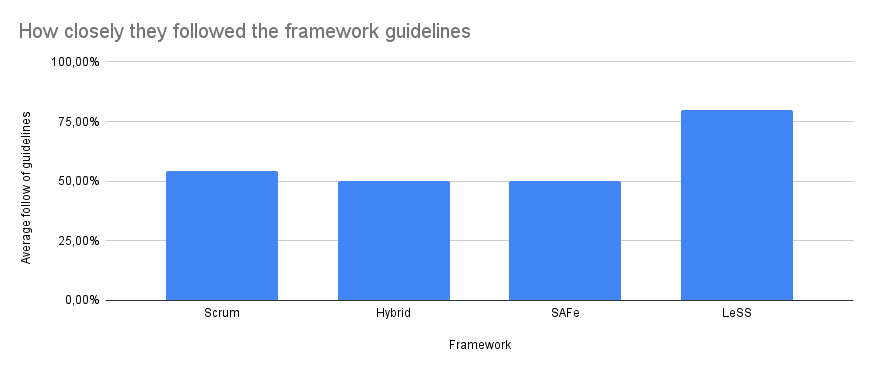
\includegraphics[width=\textwidth]{./assets/images/English/Howcloselytheyfollowedtheframeworkguidelines.png}}
        \caption{How closely they followed the framework guidelines}\label{fig:Howcloselytheyfollowedtheframeworkguidelines}
    \end{center}
\end{figure}

%\section*{Für wie gravierend halten Sie den Einfluss dieser Abweichung auf den Erfolg der Scrum Integration?}
\begin{figure}[!htb]
	\begin{center}
        \makebox[\textwidth]{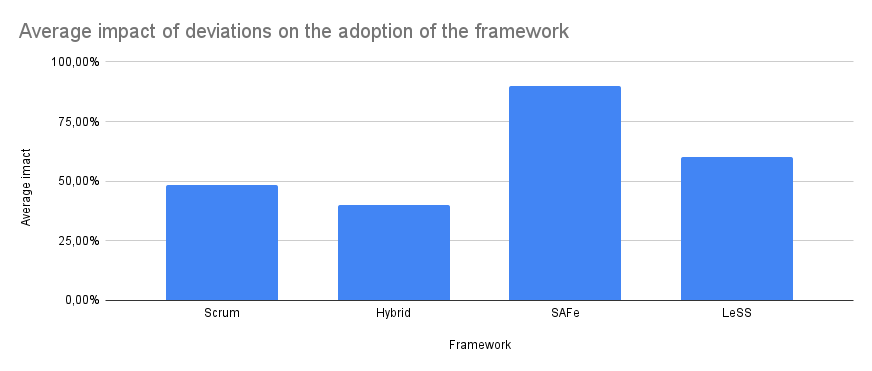
\includegraphics[width=\textwidth]{./assets/images/English/Averageimpactofdeviationsontheadoptionoftheframework.png}}
        \caption{Average impact of deviations on the adoption of the framework}\label{fig:Averageimpactofdeviationsontheadoptionoftheframework}
    \end{center}
\end{figure}

%\section*{Hatten Sie bereits Erfahrung mit einem der anderen genannten Frameworks?}
\begin{figure}[!htb]
	\begin{center}
        \makebox[\textwidth]{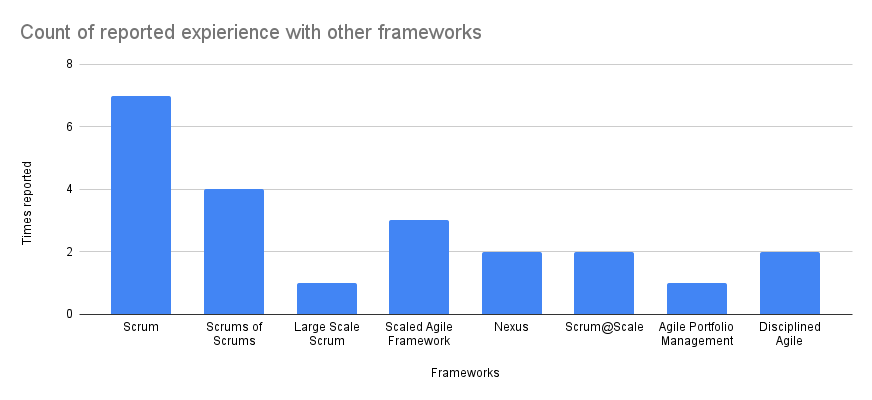
\includegraphics[width=\textwidth]{./assets/images/English/Countofreportedexpieriencewithotherframeworks.png}}
        \caption{Count of reported expierience with other frameworks}\label{fig:Countofreportedexpieriencewithotherframeworks}
    \end{center}
\end{figure}

%\section*{Welche der folgenden Methoden nutzt Ihr Unternehmen aktiv?}
\begin{figure}[!htb]
    \begin{center}
        \makebox[\textwidth]{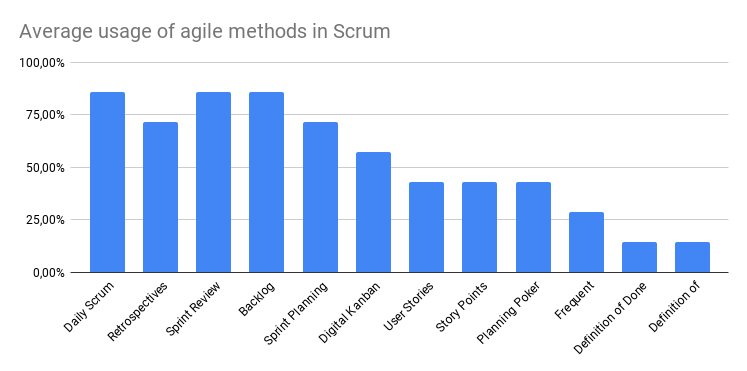
\includegraphics[width=\textwidth]{./assets/images/English/AverageusageofagilemethodsinScrum.png}}
        \caption{Average usage of agile methods in Scrum}\label{fig:AverageusageofagilemethodsinScrum}
    \end{center}
\end{figure}
\begin{figure}[!htb]
	\begin{center}
        \makebox[\textwidth]{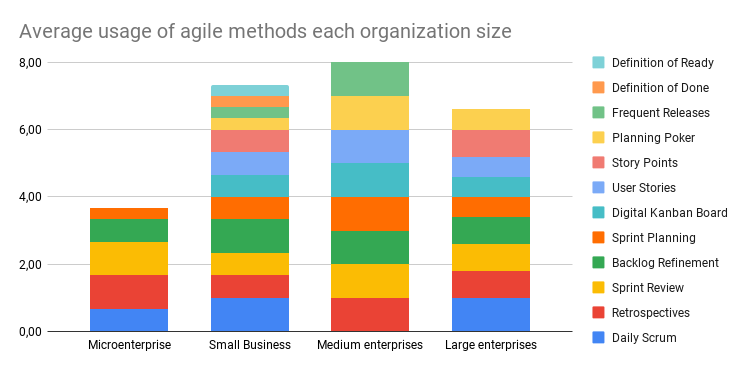
\includegraphics[width=\textwidth]{./assets/images/English/Averageusageofagilemethodseachorganizationsize.png}}
        \caption{Average usage of agile methods each organization size}\label{fig:Averageusageofagilemethodseachorganizationsize}
    \end{center}
\end{figure}
\begin{figure}[!htb]
	\begin{center}
        \makebox[\textwidth]{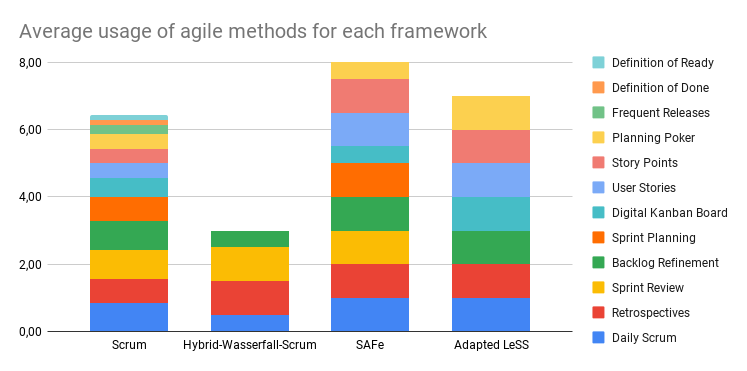
\includegraphics[width=\textwidth]{./assets/images/English/Averageusageofagilemethodsforeachframework.png}}
        \caption{Average usage of agile methods for each framework}\label{fig:Averageusageofagilemethodsforeachframework}
    \end{center}
\end{figure}

%\section*{Wie würden Sie die Expertise bewerten, die ein solches Zertifikat vermittelt?}
\begin{figure}[!htb]
    \begin{center}
        \makebox[\textwidth]{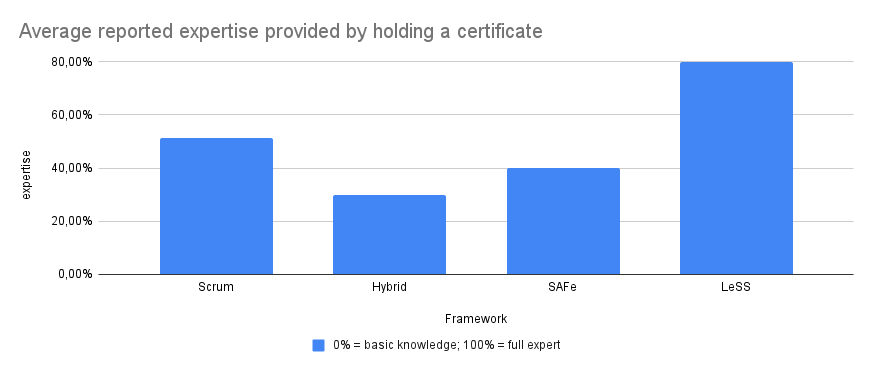
\includegraphics[width=\textwidth]{./assets/images/English/Averagereportedexpertiseprovidedbyholdingacertificate.png}}
        \caption{Average reported expertise provided by holding a certificate}\label{fig:Averagereportedexpertiseprovidedbyholdingacertificate}
    \end{center}
\end{figure}

%\section*{Wie würden Sie den Erfolg der Integration von Scrum in Ihrem Unternehmen bewerten?}
\begin{figure}[!htb]
    \begin{center}
        \makebox[\textwidth]{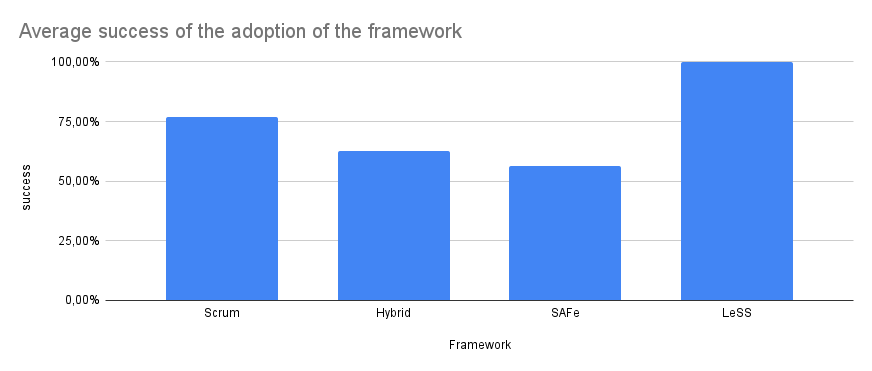
\includegraphics[width=\textwidth]{./assets/images/English/Averagesuccessoftheadoptionoftheframework.png}}
        \caption{Average success of the adoption of the framework}\label{fig:Averagesuccessoftheadoptionoftheframework}
    \end{center}
\end{figure}

%\section*{Wie schätzen Sie die Selbstorganisation und das Selbstmanagement Ihres Teams ein?}
\begin{figure}[!htb]
    \begin{center}
        \makebox[\textwidth]{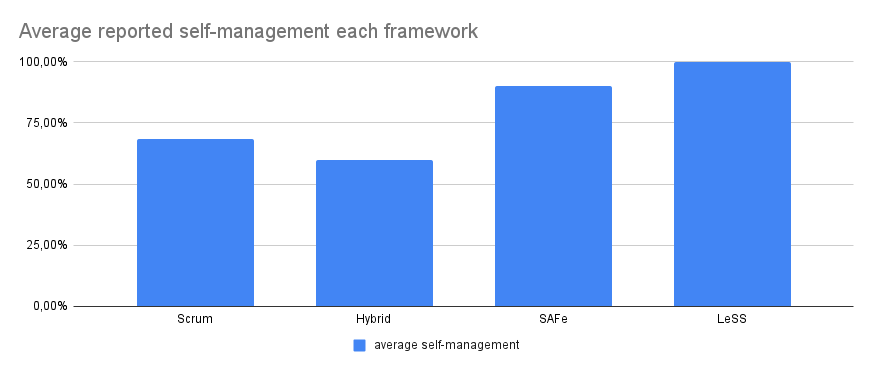
\includegraphics[width=\textwidth]{./assets/images/English/Averagereportedself-managementeachframework.png}}
        \caption{Average reported self-management each framework}\label{fig:Averagereportedself-managementeachframework}
    \end{center}
\end{figure}
\begin{figure}[!htb]
    \begin{center}
        \makebox[\textwidth]{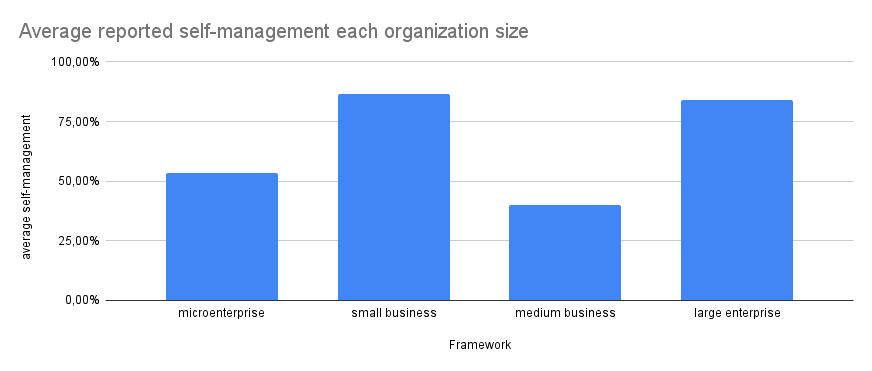
\includegraphics[width=\textwidth]{./assets/images/English/Averagereportedself-managementeachorganizationsize.png}}
        \caption{Average reported self-management each organization size}\label{fig:Averagereportedself-managementeachorganizationsize}
    \end{center}
\end{figure}

%\section*{Wie hoch ist Ihre Motivation Scrum durch ein anderes Framework zu ersetzen?}
\begin{figure}[!htb]
    \begin{center}
        \makebox[\textwidth]{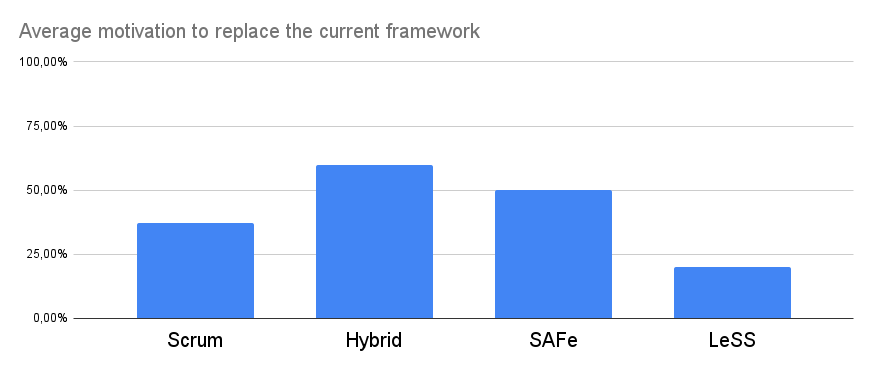
\includegraphics[width=\textwidth]{./assets/images/English/Averagemotivationtoreplacethecurrentframework.png}}
        \caption{Average motivation to replace the current framework}\label{fig:Averagemotivationtoreplacethecurrentframework}
    \end{center}
\end{figure}

%\section*{Was wären die Gründe für die Anwendung eines anderen Frameworks?}
\begin{figure}[!htb]
    \begin{center}
        \makebox[\textwidth]{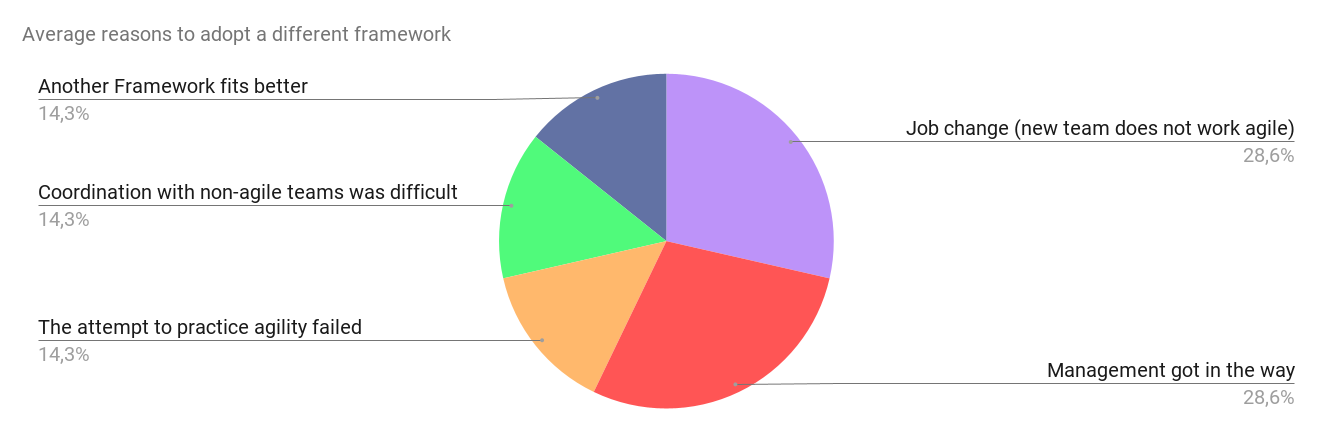
\includegraphics[width=\textwidth]{./assets/images/English/Averagereasonstoadoptadifferentframework.png}}
        \caption{Average reasons to adopt a different framework}\label{fig:Averagereasonstoadoptadifferentframework}
    \end{center}
\end{figure}

%\section*{Welche der folgenden Gründe waren es, die zur Integration von Scrum in Ihrem Unternehmen gesorgt haben?}
\begin{figure}[!htb]
    \begin{center}
        \makebox[\textwidth]{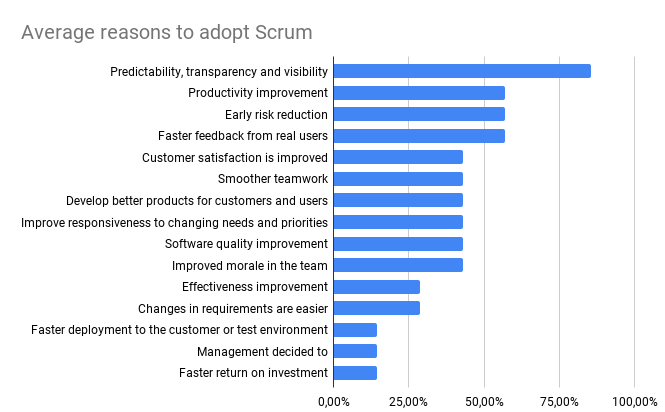
\includegraphics[width=\textwidth]{./assets/images/English/AveragereasonstoadoptScrum.png}}
        \caption{Average reasons to adopt Scrum}\label{fig:AveragereasonstoadoptScrum}
    \end{center}
\end{figure}

%\section*{Welche der folgenden Herausforderungen hatte Ihr Unternehmen bei der Integration von Scrum?}
\begin{figure}[!htb]
    \begin{center}
        \makebox[\textwidth]{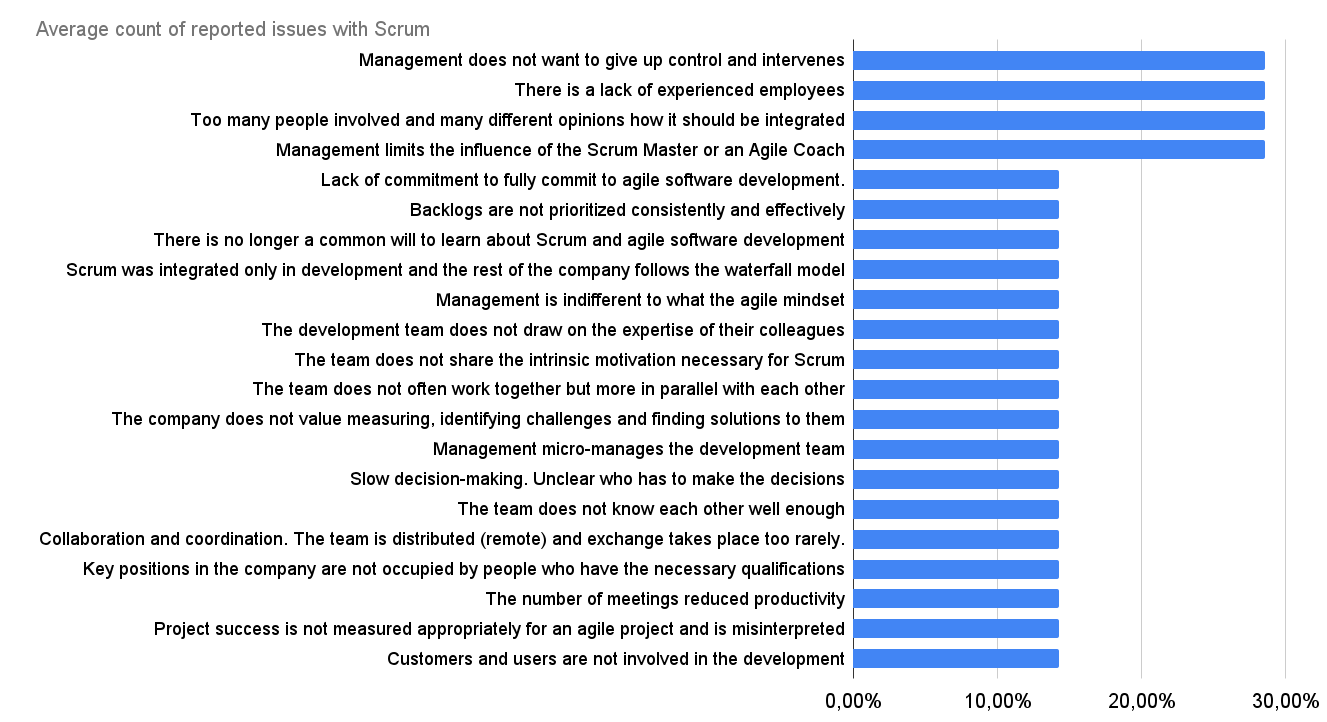
\includegraphics[width=\textwidth]{./assets/images/English/AveragecountofreportedissueswithScrum.png}}
        \caption{Average count of reported issues with Scrum}\label{fig:AveragecountofreportedissueswithScrum}
    \end{center}
\end{figure}
\begin{figure}[!htb]
    \begin{center}
        \makebox[\textwidth]{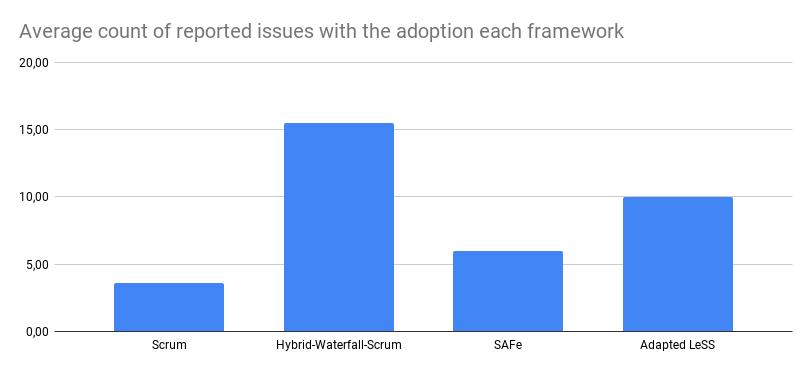
\includegraphics[width=\textwidth]{./assets/images/English/Averagecountofreportedissueswiththeadoptioneachframework.png}}
        \caption{Average count of reported issues with the adoption each framework}\label{fig:Averagecountofreportedissueswiththeadoptioneachframework}
    \end{center}
\end{figure}
\begin{figure}[!htb]
    \begin{center}
        \makebox[\textwidth]{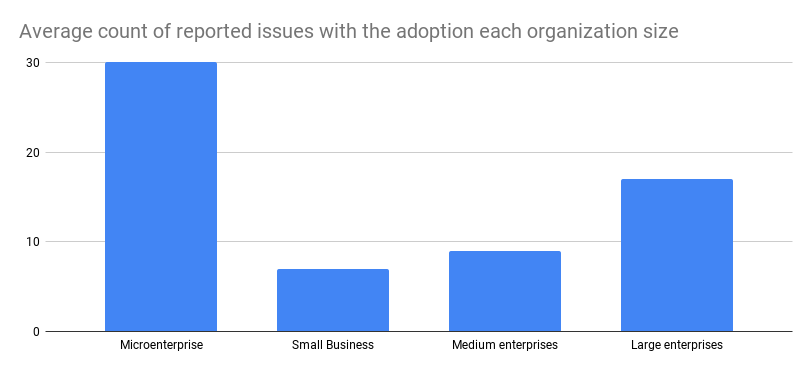
\includegraphics[width=\textwidth]{./assets/images/English/Averagecountofreportedissueswiththeadoptioneachorganizationsize.png}}
        \caption{Average count of reported issues with the adoption each organization size}\label{fig:Averagecountofreportedissueswiththeadoptioneachorganizationsize}
    \end{center}
\end{figure}

%\section*{Welche der folgenden Lösungsansätze hatte auch Ihr Unternehmen versucht?}
\begin{figure}[!htb]
    \begin{center}
        \makebox[\textwidth]{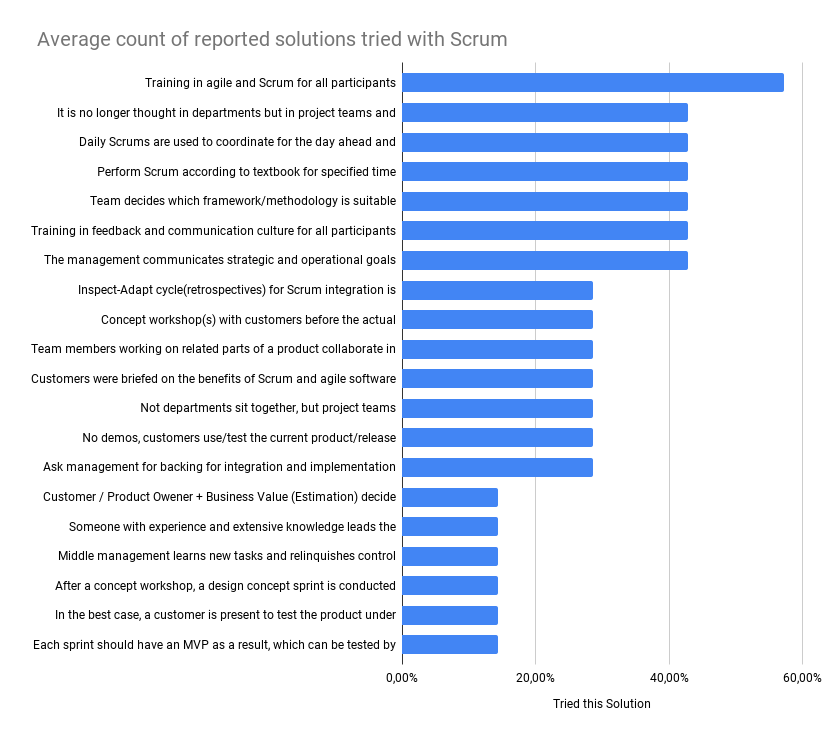
\includegraphics[width=\textwidth]{./assets/images/English/AveragecountofreportedsolutionstriedwithScrum.png}}
        \caption{Average count of reported solutions tried with Scrum}\label{fig:AveragecountofreportedsolutionstriedwithScrum}
    \end{center}
\end{figure}
\begin{figure}[!htb]
    \begin{center}
        \makebox[\textwidth]{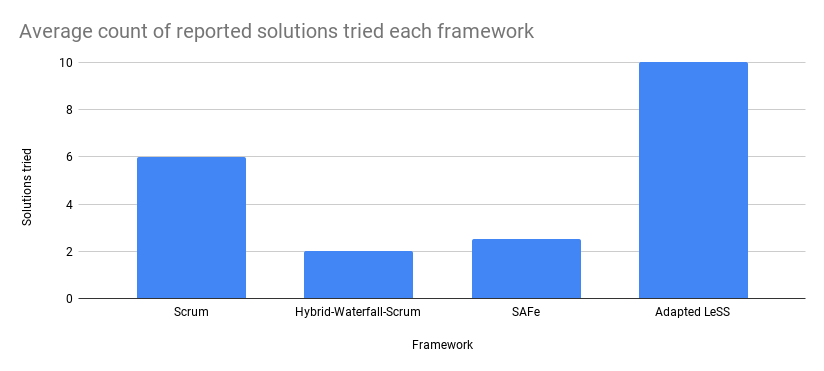
\includegraphics[width=\textwidth]{./assets/images/English/Averagecountofreportedsolutionstriedeachframework.png}}
        \caption{Average count of reported solutions tried each framework}\label{fig:Averagecountofreportedsolutionstriedeachframework}
    \end{center}
\end{figure}
\begin{figure}[!htb]
    \begin{center}
        \makebox[\textwidth]{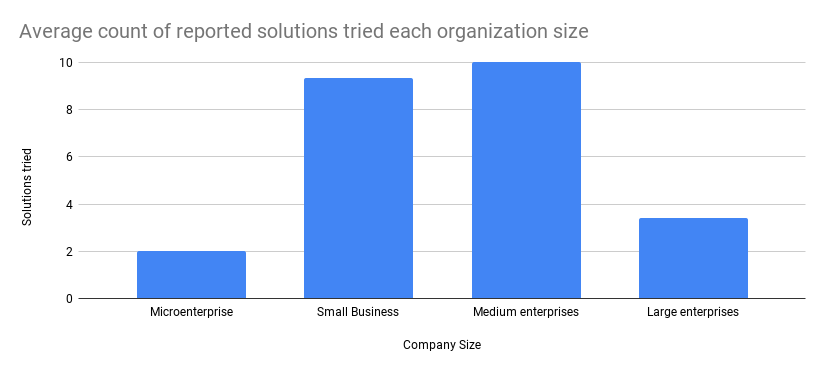
\includegraphics[width=\textwidth]{./assets/images/English/Averagecountofreportedsolutionstriedeachorganizationsize.png}}
        \caption{Average count of reported solutions tried each organization size}\label{fig:Averagecountofreportedsolutionstriedeachorganizationsize}
    \end{center}
\end{figure}

%\section*{Welche Folgen von agiler Transformation treffen auf Ihr Unternehmen zu?}
\begin{figure}[!htb]
    \begin{center}
        \makebox[\textwidth]{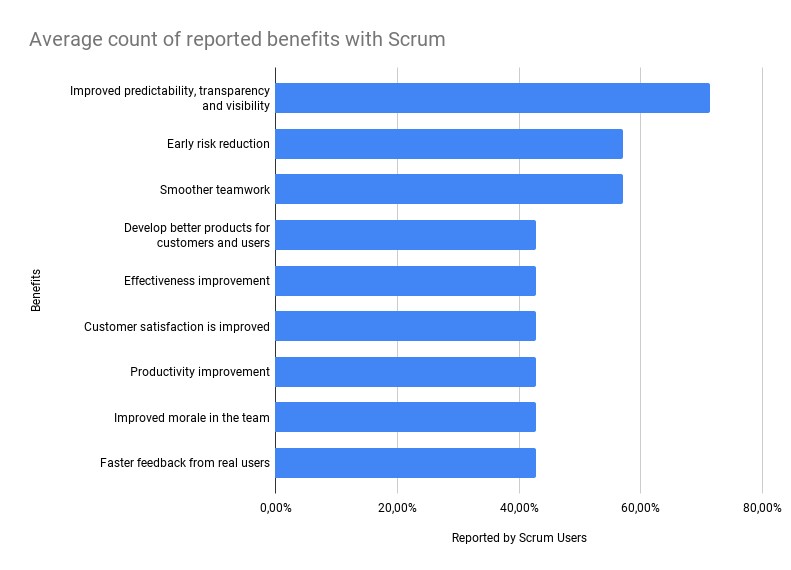
\includegraphics[width=\textwidth]{./assets/images/English/AveragecountofreportedbenefitswithScrum.png}}
        \caption{Average count of reported benefits with Scrum}\label{fig:AveragecountofreportedbenefitswithScrum}
    \end{center}
\end{figure}
\begin{figure}[!htb]
    \begin{center}
        \makebox[\textwidth]{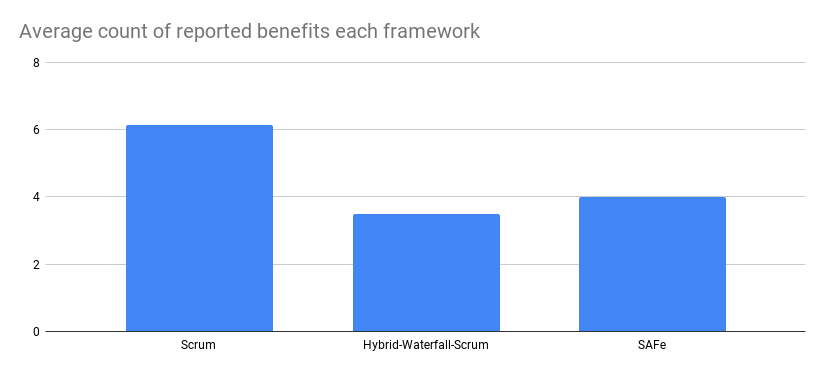
\includegraphics[width=\textwidth]{./assets/images/English/Averagecountofreportedbenefitseachframework.png}}
        \caption{Average count of reported benefits each framework}\label{fig:Averagecountofreportedbenefitseachframework}
    \end{center}
\end{figure}
\begin{figure}[!htb]
    \begin{center}
        \makebox[\textwidth]{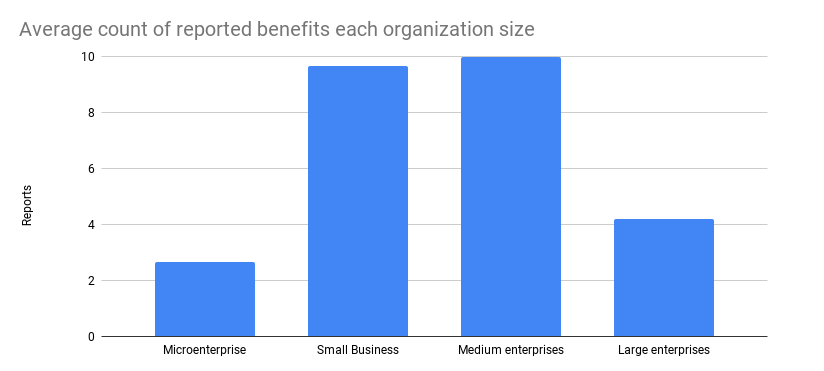
\includegraphics[width=\textwidth]{./assets/images/English/Averagecountofreportedbenefitseachorganizationsize.png}}
        \caption{Average count of reported benefits each organization size}\label{fig:Averagecountofreportedbenefitseachorganizationsize}
    \end{center}
\end{figure}



\newpage
\phantomsection%
%----------------------------------------------------------------------------------------
%	Affidavit
%----------------------------------------------------------------------------------------
%!TEX root = ../mai-joel_maximilian-bachelor_thesis.tex
%----------------------------------------------------------------------------------------
%	Debug options
%----------------------------------------------------------------------------------------
% chktex-file 2
% chktex-file 8
% chktex-file 11
% chktex-file 13
% chktex-file 18
% chktex-file 36
% chktex-file 39
% chktex-file 44
%----------------------------------------------------------------------------------------
\addcontentsline{toc}{chapter}{Affidavit}
\chapter*{Eidesstattliche Erklärung}

Ich versichere, die von mir vorgelegte Arbeit selbständig verfasst zu haben.\newline
Alle Stellen, die wörtlich oder sinngemäß aus veröffentlichten oder nicht veröffentlichten Arbeiten anderer entnommen sind, habe ich als entnommen kenntlich gemacht. Sämtliche Quellen und Hilfsmittel, die ich für die Arbeit benutzt habe, sind angegeben.\newline
Die Arbeit hat mit gleichem Inhalt bzw. in wesentlichen Teilen noch keiner anderen Prüfungsbehörde vorgelegen.
\vspace{1.5cm}

Gummersbach, Freitag 17. Februar 2023
\vspace{1cm}

%----------------------------------------------------------------------------------------
%	Insert Signature as Image here
%----------------------------------------------------------------------------------------
\begin{figure}[!ht]
	
\includegraphics[width=0.26\textwidth]{assets/images/mySignature.jpg}
\end{figure}

Joël Maximilian Mai
\newpage